% Created 2020-01-24 Fri 10:06
% Intended LaTeX compiler: pdflatex
\documentclass[presentation,aspectratio=169,smaller]{beamer}
\usepackage[utf8x]{inputenc}
\usepackage[T1]{fontenc}
\usepackage{graphicx}
\usepackage{grffile}
\usepackage{longtable}
\usepackage{wrapfig}
\usepackage{rotating}
\usepackage[normalem]{ulem}
\usepackage{amsmath}
\usepackage{textcomp}
\usepackage{amssymb}
\usepackage{capt-of}
\usepackage{hyperref}
\usepackage{color}
\usepackage[newfloat]{minted}
\usepackage[utf8]{inputenc}
\usepackage{soul}
\usepackage{unicode-math}
\usepackage{mathtools}
\usepackage[mathletters]{ucs}
\usemintedstyle{tango}
\setminted{fontsize=\scriptsize}
\setminted{mathescape=true}
\setbeamertemplate{itemize items}[circle]
\setbeamertemplate{enumerate items}[default]
\setlength{\parskip}{\baselineskip}%
\setlength{\parindent}{0pt}%
\setbeamertemplate{navigation symbols}{}%remove navigation symbols
\newcommand{\hlyellow}[1]{\colorbox{yellow!50}{$\displaystyle#1$}}
\newcommand{\hlfancy}[2]{\sethlcolor{#1}\hl{#2}}
\usetheme{default}
\author{Boris Buliga/Borys Bulyha}
\date{January 23, 2020}
\title{Out of X/Quartz}
\hypersetup{
 pdfauthor={Boris Buliga/Borys Bulyha},
 pdftitle={Out of X/Quartz},
 pdfkeywords={},
 pdfsubject={},
 pdfcreator={Emacs 28.0.50 (Org mode 9.3.1)}, 
 pdflang={English}}
\begin{document}

\maketitle
\newcommand{\mathcolorbox}[2]{%
  \begingroup
  \setlength{\fboxsep}{2pt}%
  \colorbox{#1}{$\displaystyle #2$}%
  \endgroup
}

\AtBeginSection[]{
  \begin{frame}
  \vfill
  \centering
  \begin{beamercolorbox}[sep=8pt,center,shadow=true,rounded=true]{title}
    \usebeamerfont{title}\insertsectionhead\par%
  \end{beamercolorbox}
  \vfill
  \end{frame}
}

\section{Evolution so far}
\label{sec:org285f042}

\begin{frame}[label={sec:org0693cef}]{Long time ago}
\begin{center}
\includegraphics[height=7.0cm]{images/evolution-1.png}
\end{center}

\scriptsize{www.ft.com}
\end{frame}

\begin{frame}[label={sec:org79d04b5}]{Not that far away from now}
\begin{center}
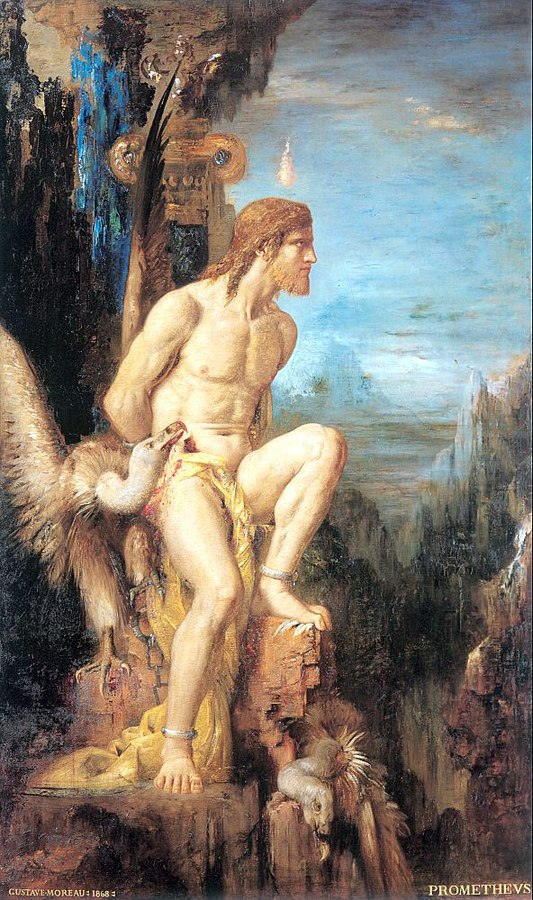
\includegraphics[height=7.0cm]{images/evolution-2.png}
\end{center}

\scriptsize{Moreau - Prometheus}
\end{frame}

\begin{frame}[label={sec:org4132d52}]{More recent events}
\begin{itemize}
\item \ldots{} important stuff happens (wine and math).
\item 33 AD -- people started to look at the bright side of life (according to MP).
\item \ldots{} math continues to evolve.
\item 1822 -- Charles Babbage designs first Analytical Engine.
\item 1840s -- Ada Lovelace writes a program for this engine to calculate
Bernoulli numbers.
\item 1936 -- Alan Turing presents the notion of a universal machine.
\item 1945 -- ENIAC, first electronic general-purpose computer is built.
\item 1950s -- COBOL, Fortran.
\item 1960s -- Douglas Engelbart creates first ever computer mouse.
\item 1971 -- Ken Thompson creates first version of Unix shell.
\item 1976 -- release of Emacs.
\item 1981 -- computers with mice in mass production.
\item 1984 -- the first release of X window server (though it's not the first one).
\item \ldots{}
\end{itemize}
\end{frame}

\begin{frame}[label={sec:org6da2b84}]{Present days}
\begin{center}
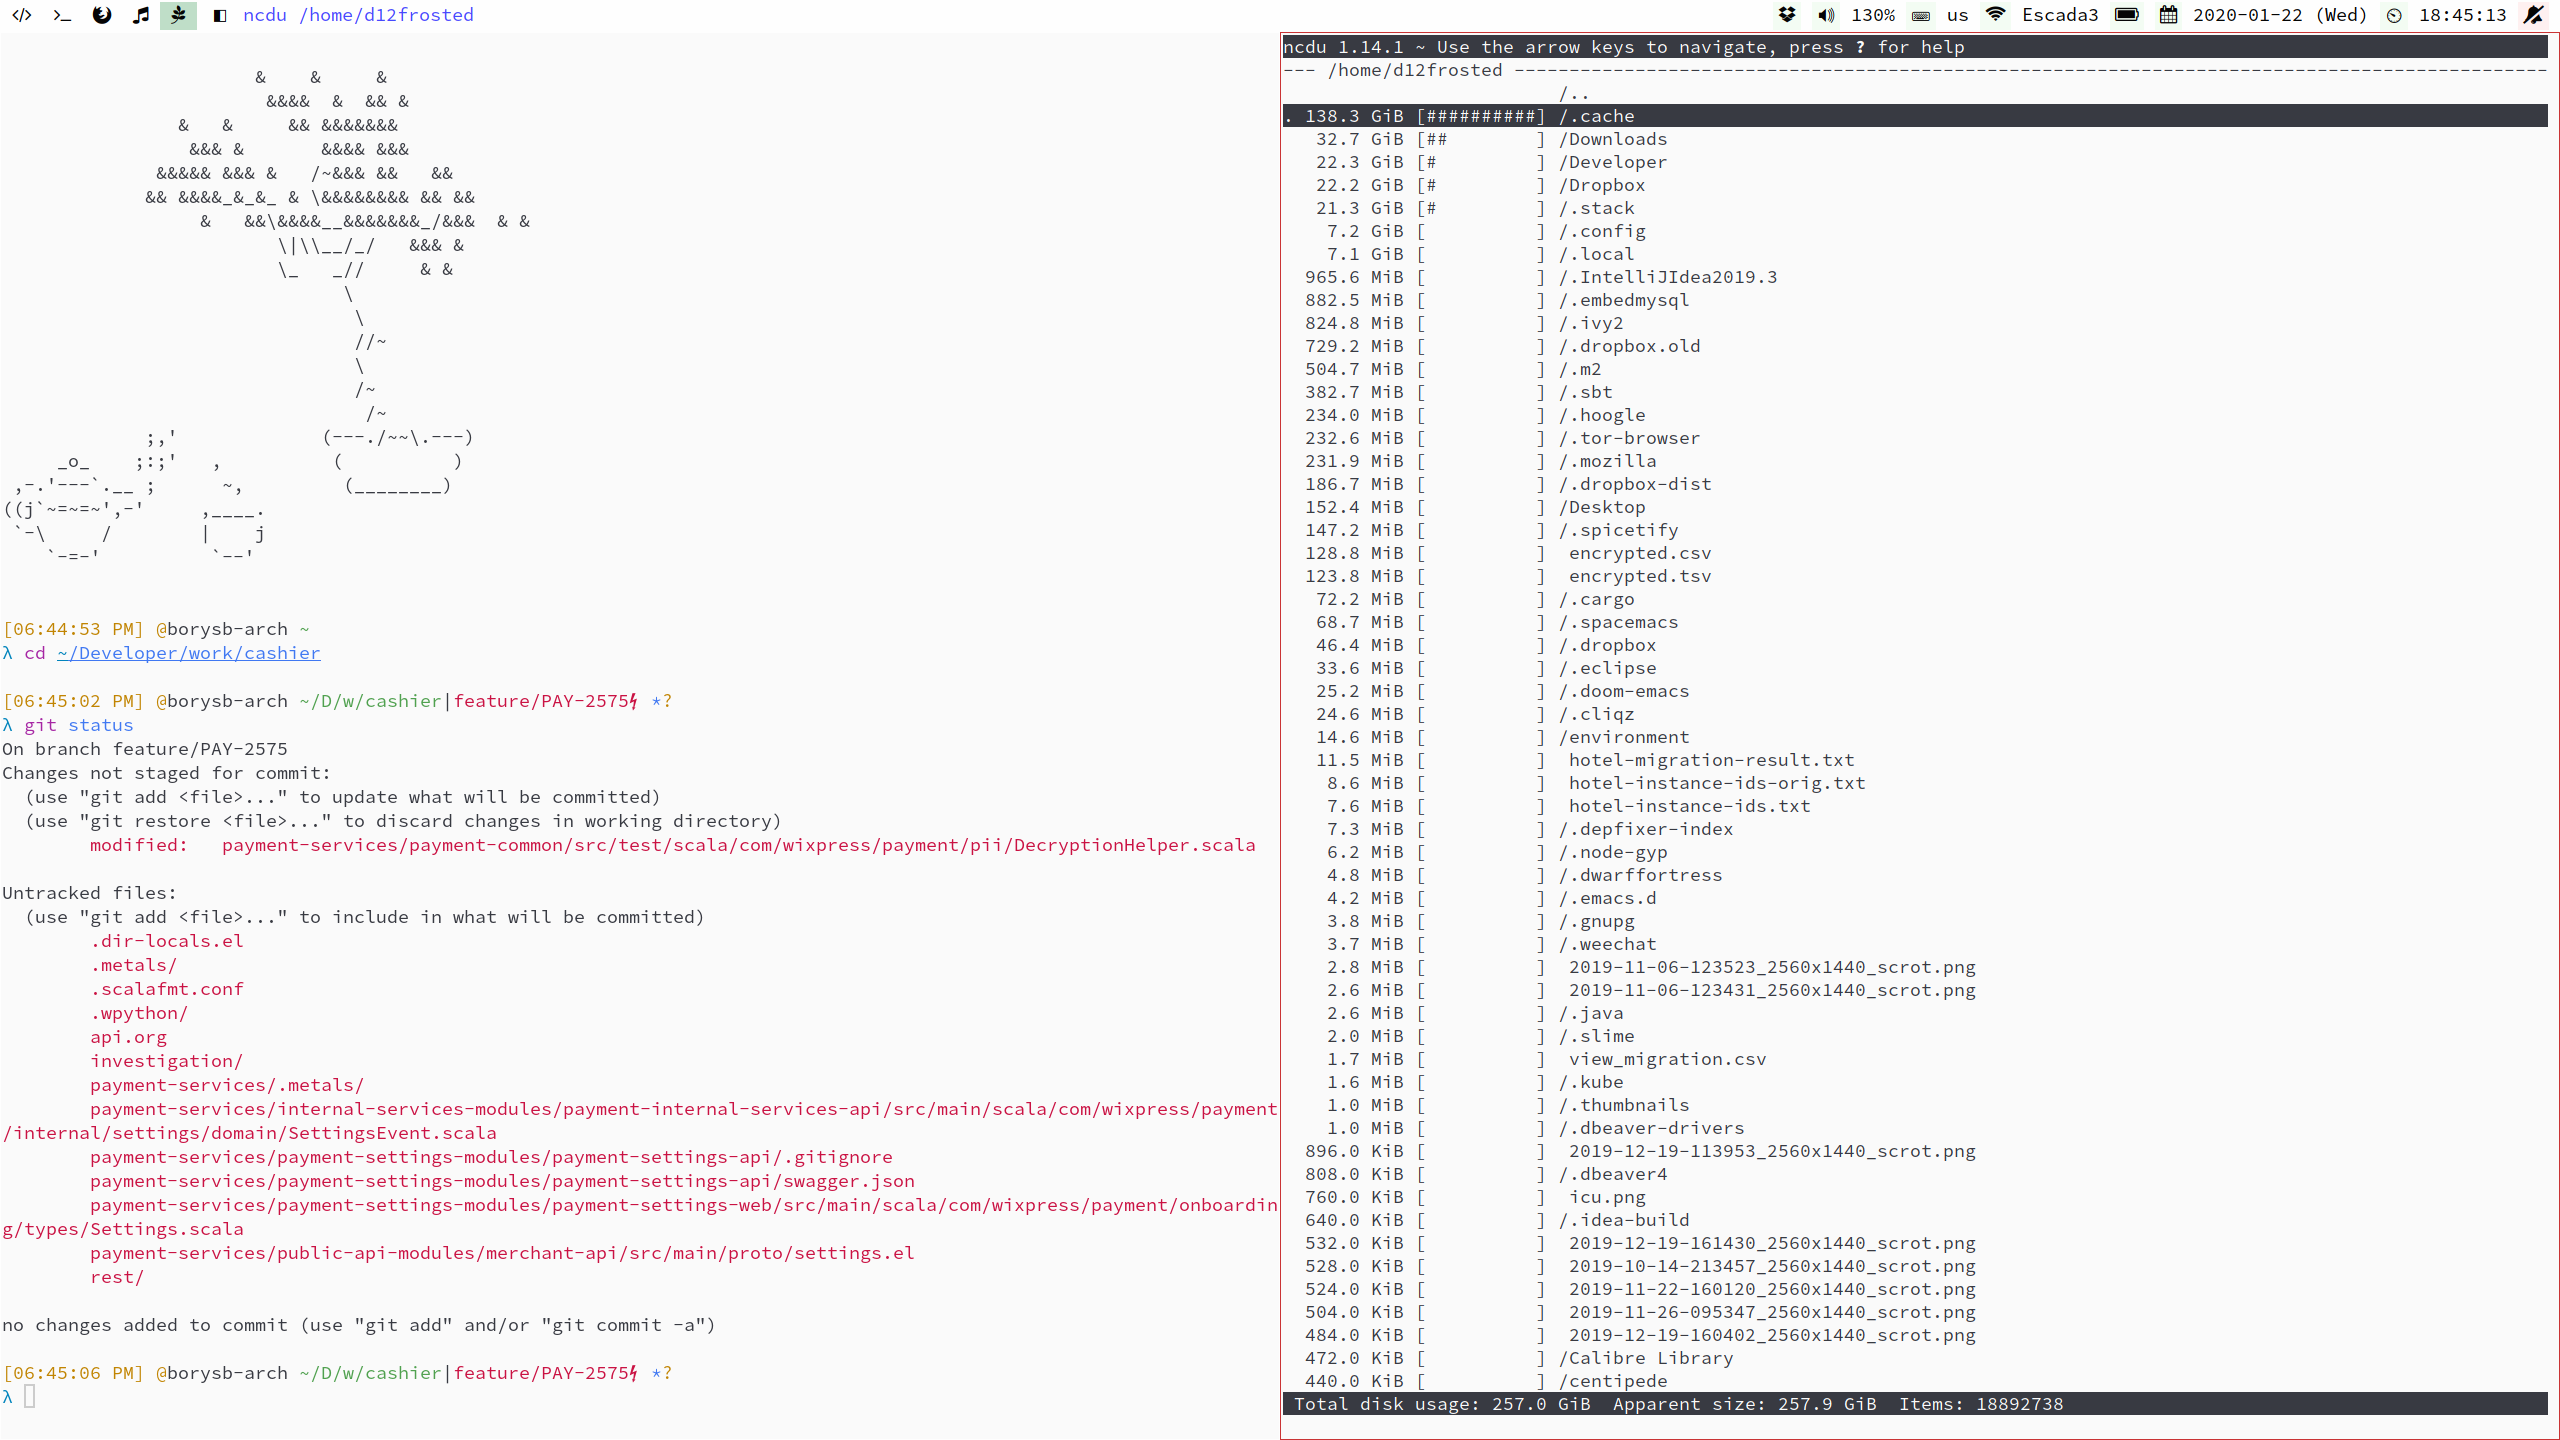
\includegraphics[height=7.0cm]{images/evolution-3.png}
\end{center}
\end{frame}

\begin{frame}[label={sec:org5036d19}]{About me}
\begin{columns}
\begin{column}{0.75\columnwidth}
\begin{itemize}
\item Server developer @Payments by Wix.
\item Haskell ↔ Emacs Lisp extremist. Whatever that means.
\item Chinese tea drinker.
\item Wine-lifestyle activist (92\% of my life).
\item @d12frosted
\end{itemize}
\end{column}

\begin{column}{0.25\columnwidth}
\begin{center}
\includegraphics[height=3.5cm]{images/boris.jpg}
\end{center}
\end{column}
\end{columns}
\end{frame}

\begin{frame}[label={sec:org7306622}]{Agenda}
\begin{itemize}
\item Shells
\item PATH
\item Basic commands
\item Being privileged
\item Piping
\end{itemize}
\end{frame}

\section{To GUI or not?}
\label{sec:org72821d8}

\begin{frame}[label={sec:org7827cf0}]{GUI motivation}
\begin{itemize}
\item GUI is usually more user friendly (≠ obvious)
\begin{itemize}
\item Explorable in a passive fashion
\item In most cases you don’t have to read documentation or excessively use DuckDuckGo
\end{itemize}
\item Some tasks are hard or nearly impossible to solve without a decent user interface
\begin{itemize}
\item Editing Video or Image
\item Real-time 3D games?
\end{itemize}
\end{itemize}
\end{frame}

\begin{frame}[label={sec:orga8d10ce}]{CLI Motivation}
\begin{itemize}
\item GUI and TUI are usually less powerful than CLI
\begin{itemize}
\item Automation
\item Composition
\end{itemize}
\item GUI is not always available
\begin{itemize}
\item X server is not started automatically (let’s greet my setup)
\item SSH
\end{itemize}
\end{itemize}
\end{frame}

\section{Unix shell}
\label{sec:orgf73c368}

\begin{frame}[label={sec:orgaccff8d},fragile]{Mushlya}
 \begin{itemize}
\item Unix shell is command-line interpreter and a scripting language.
\item Hides technical details of the OS kernel interface.
\item Everyone uses shell, but not necessarily directly.
\item 'Modern' shells:
\begin{itemize}
\item Bourne shell -- \texttt{sh}
\item Bourne-Again shell -- \texttt{bash}
\item Korn shell -- \texttt{ksh}
\item Z shell -- \texttt{zsh}; default on macOS since 10.15 Catalina
\item C shell -- \texttt{csh} or \texttt{tcsh}
\item Fish shell -- \texttt{fish}
\end{itemize}
\end{itemize}
\end{frame}

\begin{frame}[label={sec:orgd7e2775}]{Terminal emulator}
User interacts with shell using terminal emulator

\begin{itemize}
\item Terminal.app
\item iTerm
\item xterm
\item rxvt
\item kitty
\end{itemize}
\end{frame}

\begin{frame}[label={sec:orgca34690},fragile]{Binary location}
 \begin{columns}
\begin{column}{0.5\columnwidth}
\begin{minted}[]{bash}
$ command -v bash
/usr/bin/bash

$ command -v echo
/usr/bin/echo

$ command -v wixtaller
/home/d12frosted/.local/bin/wixtaller

$ command -v command
<error>
\end{minted}
\end{column}

\begin{column}{0.5\columnwidth}
\begin{minted}[]{bash}
$ which bash
/usr/bin/bash

$ which echo
/usr/bin/echo

$ which wixtaller
/home/d12frosted/.local/bin/wixtaller

$ which which
/usr/bin/which
\end{minted}
\end{column}
\end{columns}
\end{frame}

\begin{frame}[label={sec:org4d510fc},fragile]{\texttt{PATH}}
 \begin{minted}[]{bash}
$ echo $PATH
/home/d12frosted/.config/bin /home/d12frosted/.local/bin /usr/local/sbin /usr/local/bin /usr/bin
\end{minted}

\begin{minted}[]{bash}
export PATH=$HOME/.local/bin:$PATH
\end{minted}

Put in:

\begin{itemize}
\item \texttt{\$HOME/.bashrc}
\item \texttt{\$HOME/.zshrc}
\item \texttt{\$XDG\_CONFIG\_HOME/fish/config.fish}
\end{itemize}
\end{frame}

\begin{frame}[label={sec:org02fb53c},fragile]{Installing software}
 \begin{enumerate}
\item Use package manager
\begin{enumerate}
\item \texttt{brew} -- \url{https://brew.sh}
\item \texttt{pacman}
\item \texttt{apt-get}
\end{enumerate}
\item Update to the latest versions
\begin{enumerate}
\item \texttt{brew upgrade}
\item \texttt{pacman -Syu}
\item ???
\end{enumerate}
\end{enumerate}
\end{frame}

\begin{frame}[label={sec:org9839e79}]{Important}
Run command only when you understand what it does!
\end{frame}

\begin{frame}[label={sec:orgfe41e6b},fragile]{Basic commands}
 \begin{itemize}
\item \texttt{man command} - manual for command
\begin{itemize}
\item \texttt{command -{}-help}
\item \texttt{command -h}
\end{itemize}
\item \texttt{pwd} - prints working directory
\item \texttt{ls} - list files (useful options are \texttt{-l}, \texttt{-a}, \texttt{-h})
\item \texttt{cd} - change directory
\item \texttt{cat} - view file
\item \texttt{less} - view something
\item \texttt{rm} - remove file
\end{itemize}
\end{frame}

\begin{frame}[label={sec:org9d059df},fragile]{Printing and interpolation}
 \begin{minted}[]{bash}
$ echo "hello world"
hello world

$ echo "hello $USER"
hello d12frosted

$ echo 'hello $USER'
hello $USER
\end{minted}
\end{frame}

\begin{frame}[label={sec:orgd5be66e},fragile]{Redirect}
 \begin{minted}[]{bash}
$ echo "hello" > file.txt

$ cat file.txt
hello

$ echo "world" > file.txt

$ cat file.txt
world

$ cat file.txt > other-file.txt

$ echo "is huge" >> other-file.txt

$ cat other-file.txt
world
is huge
\end{minted}
\end{frame}

\begin{frame}[label={sec:org185c4e6},fragile]{Piping}
 \begin{minted}[]{bash}
$ curl --help

$ curl --help | less

$ brew install jq

$ curl https://api.coindesk.com/v1/bpi/currentprice.json
\end{minted}
\end{frame}

\begin{frame}[label={sec:org9ffea63},fragile]{Right or left}
 \begin{minted}[]{bash}
$ pacman -S hlint
error: you cannot perform this operation unless you are root.

$ sudo pacman -S hlint
\end{minted}
\end{frame}

\begin{frame}[label={sec:orgf119221},fragile]{Dollar or hash?}
 \begin{itemize}
\item \texttt{\$ command} -- execute as regular user
\item \texttt{\# command} -- execute as privileged user
\end{itemize}
\end{frame}
\section{Questions?}
\label{sec:org682f48c}
\section{Thank you}
\label{sec:orgaf4c8f0}
\end{document}
